\chapter{Evaluation}
\label{chap:eval}

To answer the research question of whether a multiple sequence alignment algorithm based solely on spaced word matches and consistency checking is able to \textbf{efficiently} provide \textbf{biologically plausible} alignments, we need to systematically evaluate and compare it to different approaches. Asserting whether the algorithm is efficient can be done by simply running it on different input sizes and comparing it to other alignment programs. However, determining whether the produced alignments are biologically plausible in order to be used in further analysis is a much harder task and in itself an active area of research \cite{edgar2010quality}. This stems from the fact that an evaluation of alignment algorithms, just like its implementation, must make simplifying assumptions about the underlying evolutionary processes. There simply is no way of \textit{"proving"} an alignment algorithm is \textit{"correct"} or even \textit{"better"} than others, since we can not know the \textit{"true"} alignment of a sequence family. However, this does not mean that we cannot make reasonable assumptions to base an evaluation on.

\section{\bb 3 alignment benchmark dataset}
\label{sec:bb}
\begin{wrapfigure}{r}{0.4\textwidth}
	\centering
	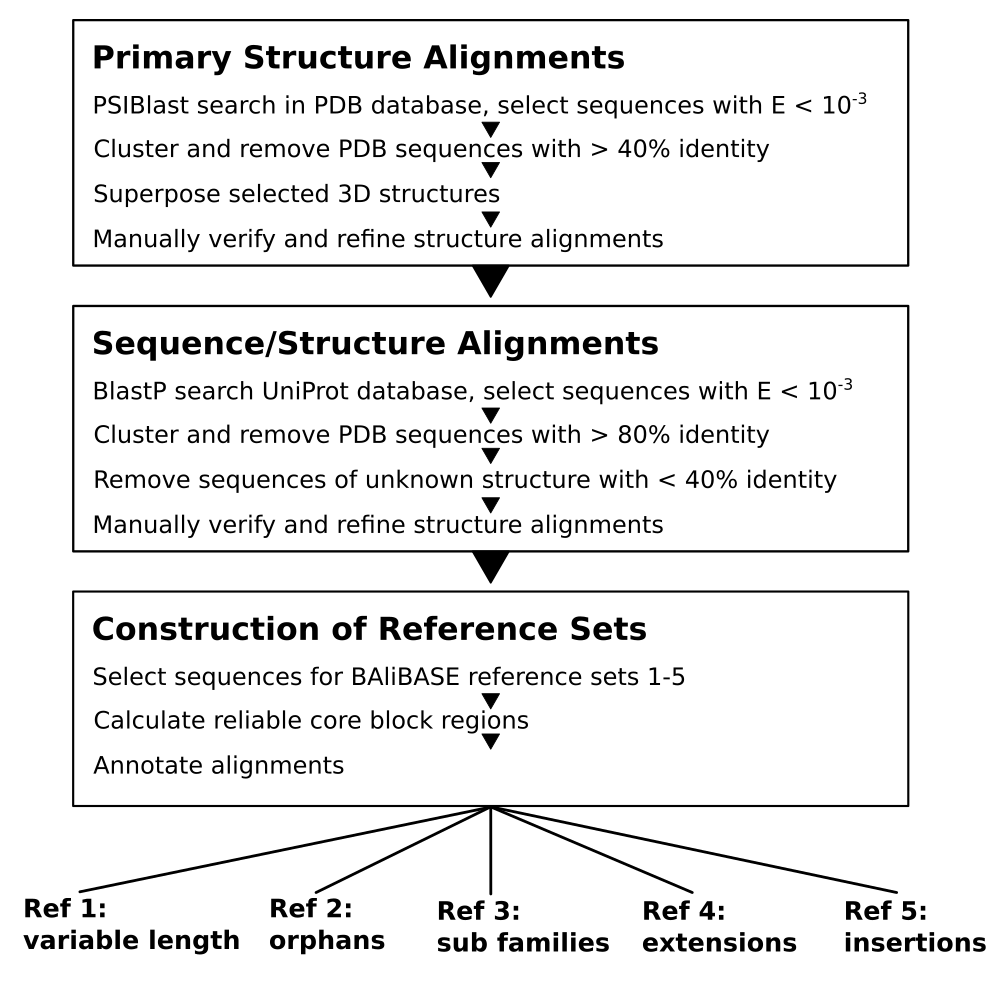
\includegraphics[width=0.5\textwidth]{./images/balibase.png}
	\caption{Semi automatic process used to establish the reference sets. Source: \cite{hundt2020praktkium}}
	\label{fig:balibase}
\end{wrapfigure}

The third version of the \bb benchmark protein alignment database has been released in 2005 and is widely employed for the comparison of multiple alignment programs \cite{thompson2005balibase, Russell2016}. It is constructed in a semi-automatic process, as shown in \cref{fig:balibase} and suitable to evaluate global and local alignment programs. The database is split into five reference sets with different characteristics representing distinctive multiple alignment problems. \\
It is divided into:



\begin{itemize}
	\item reference set 1 subset V1, for which any two sequences share <20\% identity and no internal insertions over 35 residues long
	\item reference set 1 subset V2, consisting of families with at least four equidistant sequences for which any two sequences share 20-40\% identity and no large insertions
	\item reference set 2, for which all sequences share >40\% identity and at least one 3D structure is known. Additionally, an "Orphan" sequence with <20\% identity is chosen per family
	\item for reference set 3, all sequences in the same subfamily have >40\% identity, whereas sequences from different subfamilies share <20\% identity
	\item for reference sets 4 and 5, every sequence shares at least 20\% with one other sequence, including sequences with large N/C-terminal extensions (ref 4) or internal insertions (ref 5)
\end{itemize}

\subsection{Core blocks}

Evaluating and comparing alignment programs is a challenging problem due to the uncertainty of supposedly "real" alignments of actual sequences. The \bb database marks alignment columns which can be reliably aligned as so-called "core blocks". These core blocks are calculated and manually verified, making up 19\% of the full-length sequences which are used in the evaluation of \textit{spam-align} \cite{thompson2005balibase}.

%\begin{itemize}
%    \item what are core blocks?
%    \item how are they determined and validated?
%\end{itemize}

\begin{figure}[h]
	\centering
	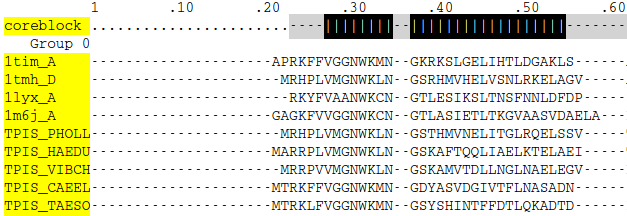
\includegraphics[width=0.8\textwidth]{./images/balibase-web.png}
	\caption{\bb web interface. Black columns indicate core blocks. \href{www.lbgi.fr/wscoperr?Balibase&FileMoi&macsimHtml&BB20006}{lbgi.fr}}
	\label{fig:bb-alignment}
\end{figure}


\section{Sum-of-pairs and column score}
Comparing the alignment output of different methods can be done by computing the sum-of-pairs and column scores.\\
Given a test alignment $A_t$ and a reference alignment $A_r$ with $M$ sequences and $N_t, N_r$ columns respectively, the sum-of-pairs and column score is defined according to Thompson et al. \cite{thompson1999comprehensive}.

\begin{mydef}[Sum-of-pairs score]
	The sum of pairs score is the ratio of correctly aligned individual residues. Formally it is defined as:
	\begin{align*}
	p_{ijk} &= \begin{cases}
	1 \text{ if residues $A_{t{_ij}}$ and $A_{t_{ik}}$ \textbf{are} aligned in $A_r$}\\
	0 \text{ otherwise}
	\end{cases} \\
	S_i &= \sum_{j=1}^{M} \sum_{k=i+1}^{M} p_{ijk} \\
	SPS &= \frac{\sum_{i=1}^{N_t} S_i} {\sum_{i=1}^{N_r} S_{r_i}}
	\end{align*}
	with $S_{r_i}$ being the number of correctly aligned residues in the reference.
\end{mydef}

\begin{mydef}[Column score]
	The column score is the ratio of correctly aligned columns. 
	\begin{align*}
	C_i &= \begin{cases}
	1 \text{ if all the residues in the i-th column are aligned correctly}\\
	0 \text{ otherwise}
	\end{cases} \\
	CS &= \frac{\sum_{i=1}^{N_t} C_i}{N_r}
	\end{align*}
	\label{def:column-score}
\end{mydef}
Note that $C_i = 1$ only if all the residues in the $i$-th column are aligned correctly and no residue belonging to this column is part of another one. For this reason, the numerator is smaller or equal to the denominator.\\
The definition of the column score is slightly different from that provided by the authors of \bb \cite{thompson1999comprehensive} but resembles the actual implementation in the included BaliScore tool and its reimplementation provided with this thesis.\\
These scores are only calculated for the core blocks of the \bb alignments, meaning that for the following evaluation $A_t$ is an alignment over the full sequences, while $A_r$ contains only the aligned residues inside the core blocks.


\section{Bali-Score}
Accompanying this thesis is a reimplementation of the \textit{bali-score} tool, which can be used to calculate the SPS and column scores given a test alignment in \code{fasta} format and a \bb reference \code{xml} file. Although some of the features which are part of the original implementation are not contained in this version, it should be significantly easier to use and install since the correct dependencies are automatically resolved and fetched by the Rust package manager.\\
The source code is available on \href{https://github.com/robinhundt/bali-score}{github.com} and, provided the current stable Rust toolchain \footnote{View \href{https://rustup.rs}{rustup.rs} for installation instruction} is available, installing the tool can simply be done by issuing \code{cargo install --path .} in the cloned repository root. For usage instructions view \code{bali-score -h}.

\section{Evaluated programs}

Answering the research question of whether the proposed approach is able to compute alignments \textit{fast} while being \textit{biologically plausible}, it is necessary to compare it against other established approaches. \textit{SpaM-Align} (where SpaM stands for \textbf{S}paced \textbf{M}atches) is the alignment program produced as part of this thesis. Although \textit{Dialign} is a dated approach, version 2.2 was released in 1999, it heavily influenced \textit{SpaM-Align} and therefore provides an interesting comparison.
The third program we compare, \textit{Mafft}, is a state of the art multiple sequence alignment tool which enables the user to choose and mix progressive, iterative and structural alignment strategies.

\subsection{SpaM-Align}
\textit{SpaM-Align} is the alignment tool which implements the greedy algorithm described in chapter \ref{chap:algorithm}. The source code is openly available\footnote{Source available at: \href{https://github.com/robinhundt/spam-align}{github.com/robinhundt/spam-align}} and the tool can be installed by executing \code{cargo install --path .} in the project root (see \code{README.md} for further details). A description of the available arguments can be displayed with \code{spam-align --help}.

\subsubsection{Evaluated patterns}
Being based on spaced word matches, \textit{SpaM-Align} requires one or more patterns \ref{def:pattern} as a parameter. In earlier work we established that it is potentially possible to identify a high ratio of homologous sites correctly, however choosing an unfit pattern set with a weight that is too high, fails to identify a large number of homologous sites. To better understand the influence that a patterns weight and the number of \textit{Don't Care} positions has, we evaluate \textit{SpaM-Align} on 84 different pattern sets. \textit{Rasbhari} by Hahn et al. \cite{hahn2016rasbhari}, a tool to generate and optimize patterns for alignment-free sequence comparison, is used to create a pattern set for every combination of weight $k \in {2, ..., 7}$ and number of \textit{Don't Care} positions $d \in {3, ..., 16}$ with the following additional parameters applied:
\begin{minted}{sh}
-m 5        # patterns per set
-q 0.05     # background match probability
-p 0.3      # match probability
-S 400      # sequence length
-H 20       # homologue region length
\end{minted}
Since \textit{Rasbhari} always places a \textit{Match} position at the beginning and end of a pattern, for a weight of 2 only patterns of the form $10^d1$ are evaluated.

\subsection{Dialign}
Dialign, described under prior work \ref{sec:dialgin}, was executed without additional parameters.

\subsection{Mafft}
\textit{Mafft} (version 7), standing for \textbf{m}ultiple \textbf{a}lignment using \textbf{f}ast \textbf{F}ourier \textbf{t}ransform, is a widely used similarity based multiple sequence alignment program employing progressive, iterative and structural strategies \cite{katoh2013mafft}.\\
Among the many different alignment options offered by \textit{Mafft}, we chose FFT-NS-1 and L-INS-i as evaluation targets. These two represent the extremes of the accuracy and speed trade-off, with FFT-NS-1 being labelled as "very fast; recommended for >2000 sequences" and L-INS-i as "probably most accurate; recommended for <200 sequences". FFT-NS-1, from now on referred to as \textit{Mafft-Fast}, is a progressive method utilizing an imprecise guide tree; L-INS-i, referred to as \textit{Mafft-Accurate} in the following, constitutes an iterative refinement method which integrates local pairwise alignment information \cite{katoh2013mafft}.

\section{Results}
Figure \ref{fig:sop-by-pattern-params} gives an overview over how different pattern configurations influence the Sum-of-Pairs score of \textit{SpaM-Align} aggregated over the whole \bb dataset and relates those to the mean Sum-of-Pairs score of Mafft-Accurate (0.867), Mafft-Fast (0.801) and Dialign (0.769). It is noteworthy that a higher weight seems to result in a better score with pattern sets of weight 7 performing the worst and sets of weight two being substantially better than those with a weight of four. The best Sum-of-Pairs score for \textit{SpaM-Align}, 0.687, is achieved with a single pattern of weight two and eleven \textit{Don't Care} positions. Interestingly increasing the number of \textit{Don't Care} positions seems to only increase the scores of the produced alignments until $d = 11$ with most of the curves plateauing after this. Unexpectedly the pattern of weight two performs worse than those with three or four \textit{Match} positions for a low number of $d$.
\begin{figure}[h]
	\centering
	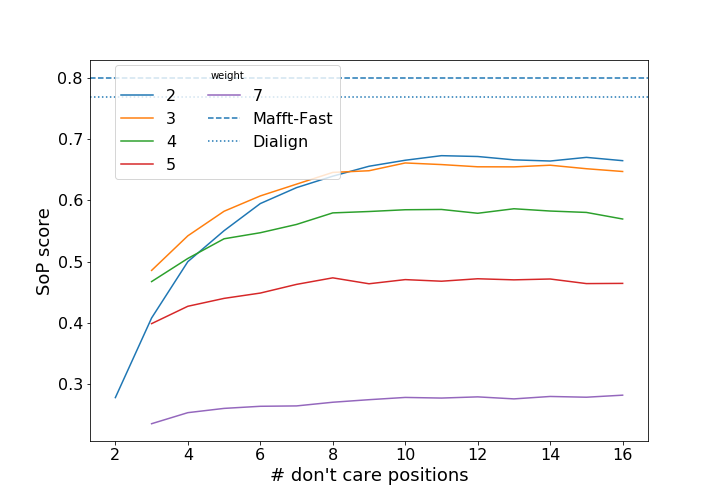
\includegraphics[width=0.8\textwidth]{../alignment-evaluation/sop-by-pattern-params.png}
	\caption{Sum-of-Pairs scores aggregated over \bb reference sets and weights and number of \textit{Don't Care} positions.}
	\label{fig:sop-by-pattern-params}
\end{figure}

Similar to figure \ref{fig:sop-by-pattern-params}, the plot \ref{fig:cs-by-pattern-params} displays the column score \ref{def:column-score} for a large number of weight and amount of \textit{Don't Care} positions, aggregated over the complete \bb data and set into context by the values for Mafft-Accurate, Mafft-Fast and Dialign. The column scores for these three points of comparison are 0.617, 0.475 and 0.450 respectively. \textit{SpaM-Align} achieves the highest column score, 0.335, with a pattern of weight two and twelve \textit{Don't Care} positions.

\begin{figure}[H]
	\centering
	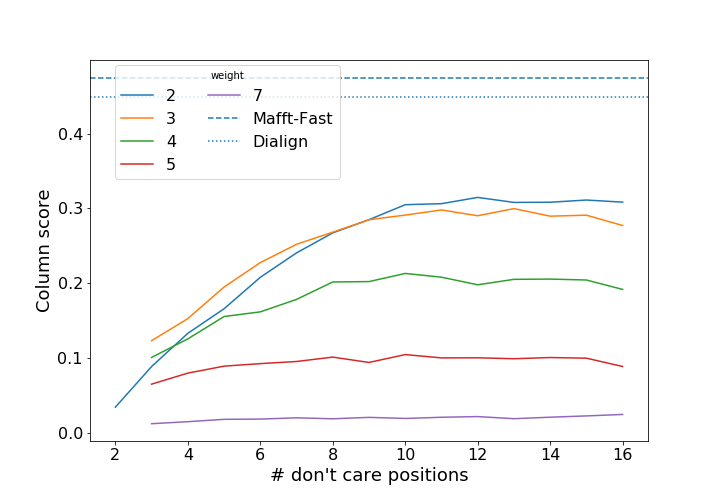
\includegraphics[width=0.9\textwidth]{../alignment-evaluation/cs-by-pattern-params.png}
	\caption{Column scores aggregated over \bb reference sets and weights.}
	\label{fig:cs-by-pattern-params}
\end{figure}

\begin{table}[h]
	\centering
	\begin{tabular}{lrrrrrr}
		\toprule
		{} &      RV11 &      RV12 &      RV20 &      RV30 &      RV40 &      RV50 \\
		\midrule
		Dialign             &  0.494482 &  0.851870 &  0.868279 &  0.739987 &  0.830939 &  0.804629 \\
		Mafft-Accurate      &  0.648562 &  0.937168 &  0.927191 &  0.862048 &  0.917403 &  0.899301 \\
		Mafft-Fast          &  0.521931 &  0.890052 &  0.885096 &  0.812195 &  0.842169 &  0.850608 \\
		SpaM-Align $k=2, d=11$ &  0.261811 &  0.751974 &  0.850375 &  0.715074 &  0.789201 &  0.733125 \\
		SpaM-Align $k=2, d=13$ &  0.247997 &  0.751732 &  0.838872 &  0.724464 &  0.770202 &  0.733305 \\
		SpaM-Align $k=3, d=10$ &  0.250701 &  0.733341 &  0.844282 &  0.714178 &  0.789304 &  0.724828 \\
		\bottomrule
	\end{tabular}
	\caption{Mean Sum-of-Pairs scores for compared programs.}
	\label{tab:sop-scores}
\end{table}

\begin{table}[h]
	\centering
	\begin{tabular}{lrrrrrr}
		\toprule
		{} &      RV11 &      RV12 &      RV20 &      RV30 &      RV40 &      RV50 \\
		\midrule
		Dialign             &  0.267504 &  0.695353 &  0.320019 &  0.411190 &  0.484710 &  0.496890 \\
		Mafft-Accurate      &  0.438860 &  0.851518 &  0.486511 &  0.657281 &  0.627038 &  0.621163 \\
		Mafft-Fast          &  0.264334 &  0.763283 &  0.340603 &  0.467281 &  0.478159 &  0.528384 \\
		SpaM-Align $k=2, d=11$ &  0.087883 &  0.548499 &  0.192057 &  0.343963 &  0.404308 &  0.350156 \\
		SpaM-Align $k=2, d=13$ &  0.068096 &  0.562437 &  0.222104 &  0.367169 &  0.397829 &  0.289876 \\
		SpaM-Align $k=3, d=10$ &  0.075997 &  0.525526 &  0.189796 &  0.334228 &  0.406251 &  0.324160 \\
		\bottomrule
	\end{tabular}
	\caption{Mean column scores for compared programs.}
	\label{tab:cs-scores}
\end{table}

But these scores represent the mean over every computed alignment in the \bb database and hide the substantial differences between the different reference sets \ref{sec:bb}.
\Cref{tab:sop-scores} shows the mean sum-of-pairs scores per subset of \bb for the benchmarked programs (only selected parameters for \textit{SpaM-Align}); \cref{tab:cs-scores} shows the mean column scores for the same programs and parameters.

\begin{figure}[h]
	\centering
	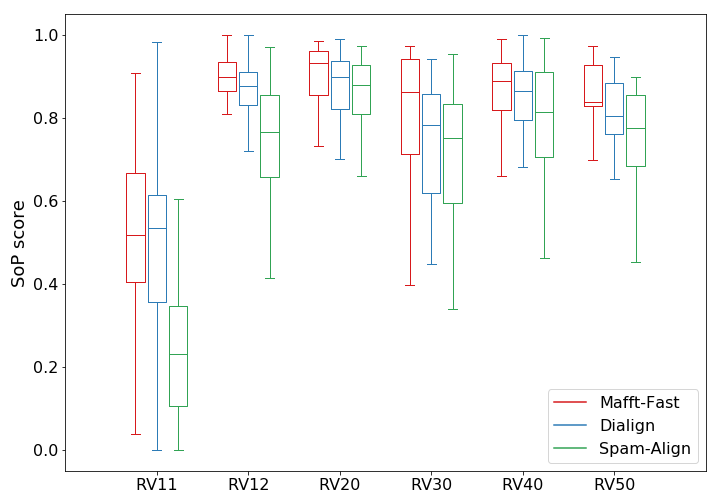
\includegraphics[width=0.8\textwidth]{../alignment-evaluation/sop-boxplot.png}
	\caption{Sum of pairs scores. Spam-Align is called with a $k = 2, d = 11$ pattern}
	\label{fig:sop-boxplot}
\end{figure}

However, even within a reference set of \bb, the Sum-of-Pairs and to a greater extent the column scores are spread widely, as can be seen by the large inter quartile ranges of the box plots \ref{fig:sop-boxplot} and \ref{fig:cs-boxplot}.

\begin{figure}[h]
	\centering
	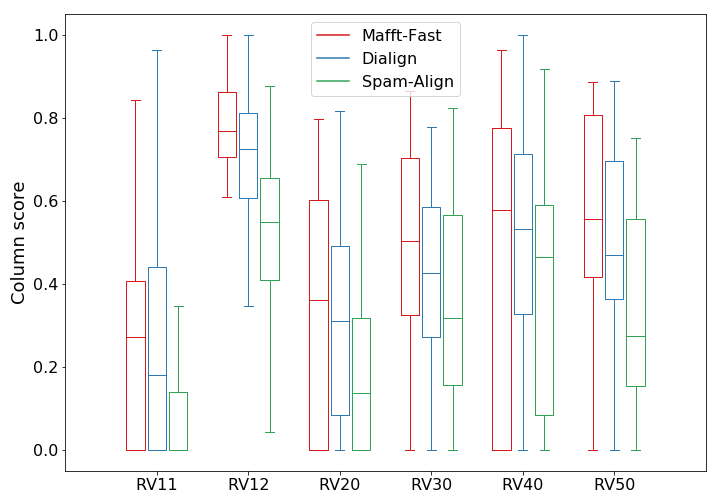
\includegraphics[width=0.8\textwidth]{../alignment-evaluation/cs-boxplot.png}
	\caption{Column scores. Spam-Align is called with a $k = 2, d = 11$ pattern.}
	\label{fig:cs-boxplot}
\end{figure}

\subsection{Execution times}

Looking at figure \ref{fig:time-by-patterns}, we see that the execution time of \textit{SpaM-Align} is significantly better than that of \textit{Dialign} (mean execution time of 26.5 seconds) and \textit{Mafft-Accurate} (mean of 16.3 second) lying between 100 ms and 500 ms depending on the weight and number of \textit{Don't Care} positions in the provided pattern set. For pattern sets with a weight of three or more, \textit{SpaM-Align} executes even faster than the speed optimized strategy \textit{Mafft-Fast} (mean of 431 ms).\\
However \cref{tab:exec-times} reveals that although \textit{SpaM-Align} only takes 5ms - 20ms on the reference sets RV11 and RV12 containing smaller sequences, compared 217ms and 254ms for \textit{Mafft-Fast}, the execution time on the larger sequences of RV30 is more than twice as \textit{Mafft-Fast} which aligns them, on average, in 455ms.

\begin{figure}[h]
	\centering
	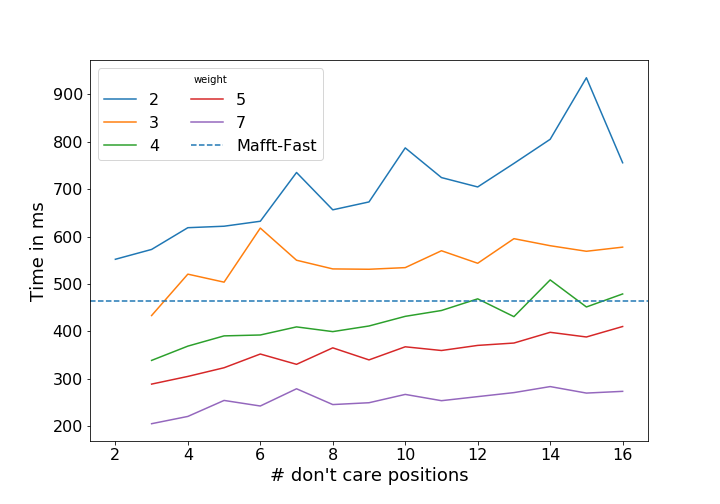
\includegraphics[width=0.9\textwidth]{../alignment-evaluation/time-by-pattern-params.png}
	\caption{Mean execution times in ms.}
	\label{fig:time-by-patterns}
\end{figure}

\begin{table}[h]
	\centering
	\begin{tabular}{lrrrrrr}
		\toprule
		{} &  RV11 &  RV12 &   RV20 &   RV30 &   RV40 &   RV50 \\
		\midrule
		Dialign             &   543 &  1626 &  40116 &  85923 &  22494 &  23141 \\
		Mafft-Accurate      &   892 &  1276 &  14676 &  25992 &  33743 &  26462 \\
		Mafft-Fast          &   217 &   254 &    425 &    455 &    705 &    559 \\
		SpaM-Align $k=2, d=11$ &     5 &    18 &    592 &   1309 &    270 &    323 \\
		SpaM-Align $k=2, d=13$ &     5 &    18 &    609 &   1338 &    279 &    340 \\
		SpaM-Align $k=3, d=10$ &     5 &    15 &    485 &   1024 &    188 &    222 \\
		\bottomrule
	\end{tabular}
	\caption{Mean execution times for compared programs}
	\label{tab:exec-times}
\end{table}
